% =========================================================
% WCCI 2026 -- A0 Poster
% Edge-Cell Graph Encoding and Fixed-Point Arithmetic
% for FPGA Growing Neural Gas
% Build: pdflatex poster.tex  (run twice)
% =========================================================
\documentclass[25pt, a0paper, portrait, margin=0mm, innermargin=15mm,
               blockverticalspace=15mm, colspace=15mm, subcolspace=8mm]{tikzposter}

\usepackage[utf8]{inputenc}
\usepackage{amsmath,amssymb,amsfonts}
\usepackage{graphicx}
\usepackage{booktabs}
\usepackage{array}
\usepackage{multirow}
\usepackage{tikz}
\usetikzlibrary{arrows.meta, positioning, shapes.geometric, calc}

% ---------- Color palette ----------
\definecolor{tmublue}{HTML}{0B3D6B}     % deep blue
\definecolor{tmuaccent}{HTML}{1B7FB8}   % mid blue
\definecolor{tmured}{HTML}{C0392B}      % accent red
\definecolor{tmugreen}{HTML}{1E8449}    % accent green
\definecolor{tmugray}{HTML}{ECF1F5}     % light bg
\definecolor{tmudark}{HTML}{17252E}

% ---------- Theme ----------
\usetheme{Default}
\usecolorstyle{Denmark}

\colorlet{titlefgcolor}{white}
\colorlet{titlebgcolor}{tmublue}
\colorlet{blocktitlebgcolor}{tmublue}
\colorlet{blocktitlefgcolor}{white}
\colorlet{backgroundcolor}{white}
\colorlet{framecolor}{tmublue}
\colorlet{notebgcolor}{tmured}
\colorlet{notefgcolor}{white}

% block style
\useblockstyle{Default}

% ---------- Custom helper commands ----------
\newcommand{\kw}[1]{\textcolor{tmublue}{\textbf{#1}}}
\newcommand{\hl}[1]{\textcolor{tmured}{\textbf{#1}}}

% =========================================================
\title{\parbox{0.95\textwidth}{\centering
       Edge-Cell Graph Encoding and Fixed-Point Arithmetic\\[6pt]
       for FPGA Growing Neural Gas}}
\author{Teuku Zikri Fatahillah$^{1}$ \quad Raditya Artha Rochmanto$^{1,2}$ \quad
        Achmad Fahrul Aji$^{1,2}$ \quad Anhar Risnumawan$^{1,3}$ \quad
        Chyan Zheng Siow$^{1,4}$ \quad Naoyuki Kubota$^{1}$}
\institute{$^{1}$Tokyo Metropolitan University, Japan \quad
        $^{2}$Politeknik Negeri Semarang, Indonesia \quad
        $^{3}$Politeknik Elektronika Negeri Surabaya, Indonesia \quad
        $^{4}$Changsha Cultural and Creative Arts Vocational College, China}

\begin{document}
\maketitle[width=810mm]

% =========================================================
\begin{columns}

% =====================  LEFT COLUMN  =====================
\column{0.5}

% ---------- Motivation ----------
\block{Motivation \& Problem}{
\large
Edge robots, micro-UAV swarms, and field devices need \kw{on-board unsupervised
adaptation} (topology formation, novelty detection) but cannot stream raw data to
the cloud. Learning must run \kw{locally} with \kw{bounded memory} and
\kw{deterministic per-sample timing}.

\vspace{4mm}
\textbf{Growing Neural Gas (GNG)} is ideal --- it learns data topology
incrementally, sample-by-sample, with no labels or retraining. But classic GNG
clashes with small-FPGA limits:
\begin{itemize}
  \item \hl{Dense adjacency matrix} scales $O(N^2)$: a $40\times40$ 8-bit matrix
        needs \hl{1{,}600\,B} --- it dominates BRAM.
  \item \hl{Floating-point} arithmetic needs FPU blocks or slow iterative units.
\end{itemize}

\vspace{3mm}
\begin{tikzfigure}
  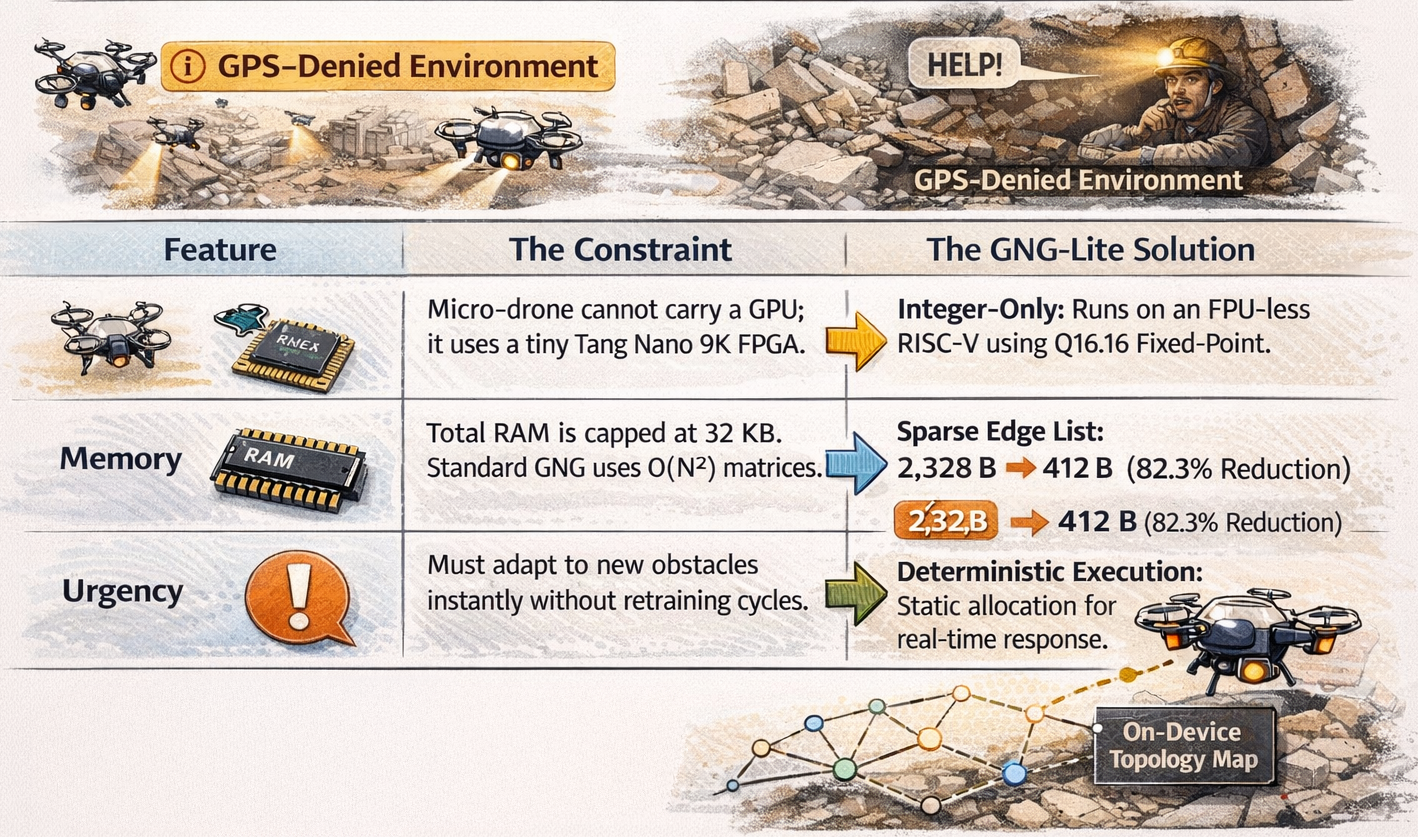
\includegraphics[width=0.92\linewidth]{problem.png}
\end{tikzfigure}
}

% ---------- Contributions ----------
\block{Our Contributions}{
\large
A fully integer, single-FSM GNG engine in synthesizable VHDL on the
\kw{Sipeed Tang Nano 9K (Gowin GW1NR-9C)} --- \kw{no soft-core CPU, no FPU}.
\begin{enumerate}
  \item \kw{Edge-cell encoding}: upper-triangular half-adjacency as 8-bit
        \emph{age+1} values (0 = no edge). \hl{780\,B} vs.\ 1{,}600\,B.
  \item \kw{Shift-based Q8/Q16} learning rates $\Rightarrow$ single-cycle DSP
        multiplies, no FPU.
  \item \kw{Fused update pass}: error decay + edge aging + neighbor move +
        pruning in \emph{one} sequential scan.
  \item \kw{Degree counters} for $O(N_{\max})$ isolated-node detection.
\end{enumerate}
}

% ---------- GNG Algorithm ----------
\block{GNG Algorithm Core}{
\large
Maintain a graph $G=(V,E)$ with weight vectors $w_i\in\mathbb{R}^2$. For each
input sample $\xi$:
\begin{enumerate}
  \item Find winner $s_1=\arg\min_i\|\xi-w_i\|^2$ and runner-up $s_2$.
  \item Accumulate / decay winner error; move $s_1$:
        $w_{s_1}\!\gets\! w_{s_1}+\epsilon_w(\xi-w_{s_1})$.
  \item Age edges of $s_1$; move neighbours; \kw{prune over-age} edges.
  \item Connect $(s_1,s_2)$, reset age $=0$.
  \item Every $\lambda$ steps insert node $r$ at the highest-error region;
        split the error.
\end{enumerate}
}

% ---------- Architecture ----------
\block{FPGA Architecture}{
\large
Single synchronous \kw{FSM datapath} at \kw{27\,MHz} (crystal, no PLL). Three
BRAMs: node, edge, dataset. \kw{80-bit node word}:
\[
\underbrace{x}_{16}\,\underbrace{y}_{16}\,\underbrace{\text{act}}_{1}\,
\underbrace{\text{deg}}_{8}\,\underbrace{\text{err}}_{32}
\]
\vspace{-4mm}

\begin{center}
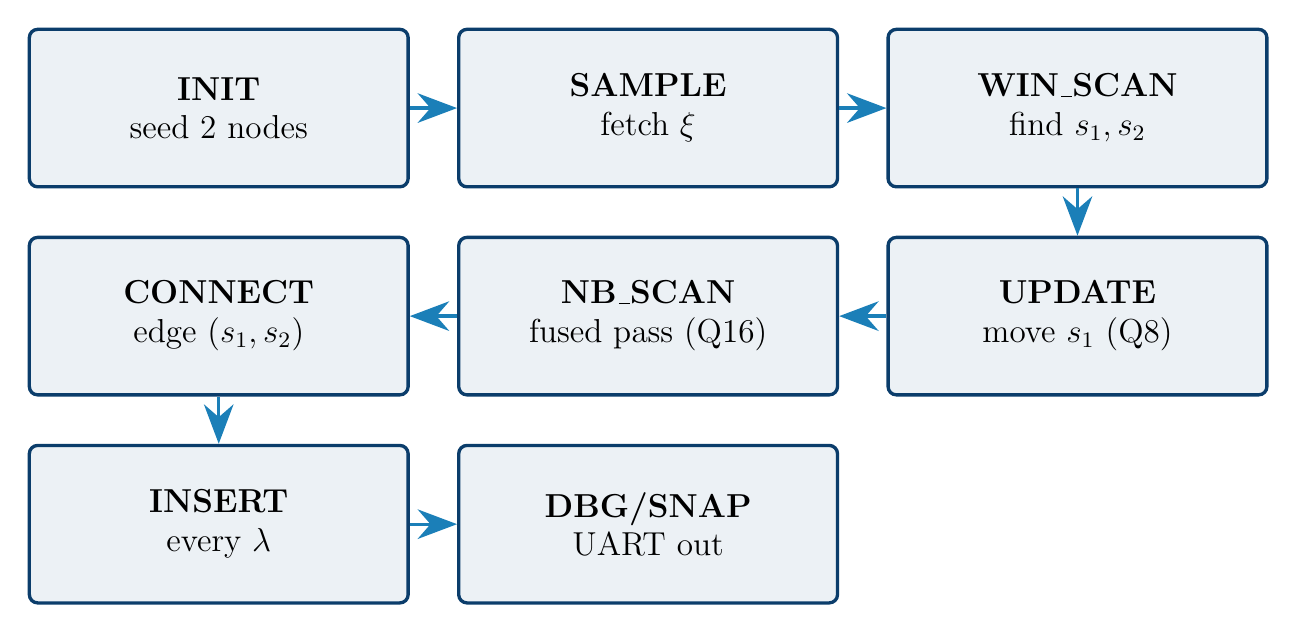
\begin{tikzpicture}[
   font=\large,
   node distance=6mm,
   box/.style={rectangle, rounded corners=3pt, draw=tmublue, very thick,
               fill=tmugray, text width=46mm, align=center,
               minimum height=20mm, inner sep=3pt},
   arr/.style={-{Stealth[length=5mm]}, very thick, tmuaccent}]
 \node[box] (init)  {\textbf{INIT}\\seed 2 nodes};
 \node[box, right=of init] (samp) {\textbf{SAMPLE}\\fetch $\xi$};
 \node[box, right=of samp] (win)  {\textbf{WIN\_SCAN}\\find $s_1,s_2$};
 \node[box, below=of win]  (upd)  {\textbf{UPDATE}\\move $s_1$ (Q8)};
 \node[box, left=of upd]   (nb)   {\textbf{NB\_SCAN}\\fused pass (Q16)};
 \node[box, left=of nb]    (con)  {\textbf{CONNECT}\\edge $(s_1,s_2)$};
 \node[box, below=of con]  (ins)  {\textbf{INSERT}\\every $\lambda$};
 \node[box, right=of ins]  (dbg)  {\textbf{DBG/SNAP}\\UART out};
 \draw[arr] (init) -- (samp);
 \draw[arr] (samp) -- (win);
 \draw[arr] (win)  -- (upd);
 \draw[arr] (upd)  -- (nb);
 \draw[arr] (nb)   -- (con);
 \draw[arr] (con)  -- (ins);
 \draw[arr] (ins)  -- (dbg);
\end{tikzpicture}
\end{center}
Each BRAM read-modify-write takes $\ge 3$ cycles (address, wait, evaluate).
}

% =====================  RIGHT COLUMN  ====================
\column{0.5}

% ---------- Edge-cell encoding (KEY) ----------
\block{Key Idea: Edge-Cell Encoding}{
\large
Store only the \kw{upper triangle} of the undirected adjacency, one byte per
potential edge, with an \kw{age+1} code:
\[
E_{\text{cells}}=\frac{N_{\max}(N_{\max}-1)}{2}
   =\frac{40\times39}{2}=\hl{780\ \text{bytes}}
\]
\begin{itemize}
  \item \texttt{cell}$=0$ : no edge \quad\textbullet\quad
        \texttt{cell}$=v>0$ : active, true age $=v-1$.
  \item No separate \emph{active} bit; over-age prune = one compare
        (\texttt{v > 51}).
  \item Linear index
        $\texttt{idx}(i,j)=\tfrac{i(2N_{\max}-i-1)}{2}+(j-i-1)$, $i<j$.
\end{itemize}

\vspace{3mm}
\innerblock{Fused NB\_SCAN Pass}{
\large One sequential scan over $N_{\max}$ slots folds together:
\kw{global error decay} $+$ \kw{edge aging} $+$ \kw{neighbor movement} $+$
\kw{over-age pruning}, replacing a separate full-array decay sweep.
}
}

% ---------- Fixed-point ----------
\block{Integer Fixed-Point Arithmetic}{
\large
16-bit signed coordinates in $[-1000,1000]$ (min-max norm $\times 1000$).

\textbf{Distance} maps onto $9\times9$ DSPs, no overflow:
\[
d^2=\Delta x^2+\Delta y^2\ \ (\text{35-bit unsigned})
\]
\textbf{Winner (Q8)} and \textbf{neighbor (Q16)} moves use shift-scaled rates:
\[
\Delta x_{s_1}\!=\!\Big\lfloor\tfrac{77\,(\xi_x-x_{s_1})}{2^{8}}\Big\rfloor
\ (\epsilon_w\!\approx\!0.301),\quad
\Delta x_{n}\!=\!\Big\lfloor\tfrac{66\,(\xi_x-x_{n})}{2^{16}}\Big\rfloor
\ (\epsilon_n\!\approx\!0.001)
\]
\textbf{Error decay} is a single right-shift:
$\mathrm{err}_n \mathrel{-}=\mathrm{err}_n\!\gg\!8$
$(\beta\approx255/256)$ --- no multiplier needed.
}

% ---------- Results: tables ----------
\block{Results}{
\large
\begin{minipage}[t]{0.48\linewidth}
\centering
\textbf{Memory footprint} ($N_{\max}=40$)\\[2mm]
\begin{tabular}{lrr}
\toprule
 & Edge & Total \\
\midrule
Dense adj. & 1600\,B & 2000\,B \\
\textbf{Edge-cell} & \hl{780\,B} & \hl{1180\,B} \\
\midrule
Reduction & \textbf{51\%} & \textbf{41\%} \\
\bottomrule
\end{tabular}
\end{minipage}\hfill
\begin{minipage}[t]{0.48\linewidth}
\centering
\textbf{FPGA utilization} (GW1NR-9C)\\[2mm]
\begin{tabular}{lrr}
\toprule
Resource & Used & \% \\
\midrule
LUT      & 3205 & 38\% \\
FF       & 1408 & 22\% \\
BSRAM    &    6 & 24\% \\
DSP      &    5 & 50\% \\
\bottomrule
\end{tabular}
\end{minipage}

\vspace{6mm}
\centering
\textbf{Topology quality \& runtime (27\,MHz)}\\[2mm]
\begin{tabular}{lccccc}
\toprule
Dataset & Nodes & Edges & QE & TE & $\mu$s/sample \\
\midrule
Two Moons          & 40 & 37 & 0.146 & 0.00 & 624 \\
Concentric Circles & 40 & 40 & 0.200 & 0.04 & 627 \\
\bottomrule
\end{tabular}\\[2mm]
\large Deterministic $\sim$625\,$\mu$s/sample $\Rightarrow$ $\sim$1{,}600 samples/s.
}

% ---------- Figures ----------
\block{Learned Topologies}{
\begin{tikzfigure}[Two Moons (left) and Concentric Circles (right): learned GNG graph, $N_{\max}=40$.]
  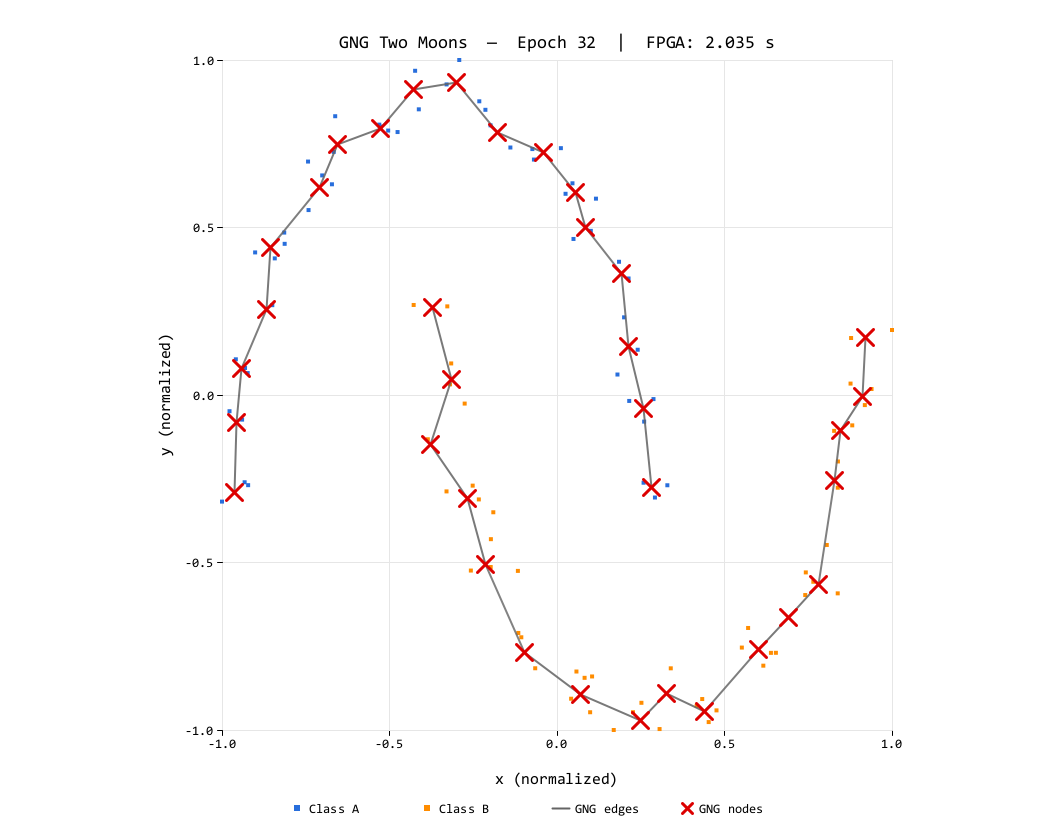
\includegraphics[width=0.40\linewidth]{two_moons_result.png}\hspace{6mm}
  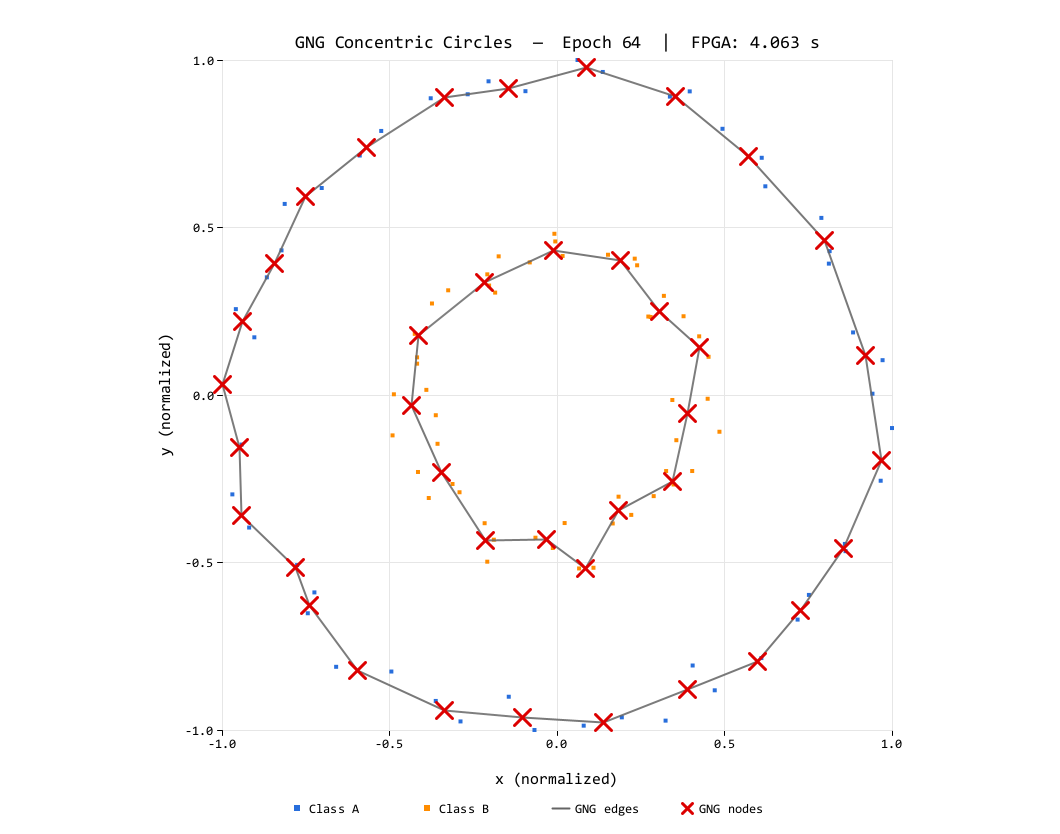
\includegraphics[width=0.40\linewidth]{concentric_circles_result.png}
\end{tikzfigure}
\vspace{2mm}
\begin{tikzfigure}[Training dynamics: node/edge growth, QE convergence, TE vs.\ epoch.]
  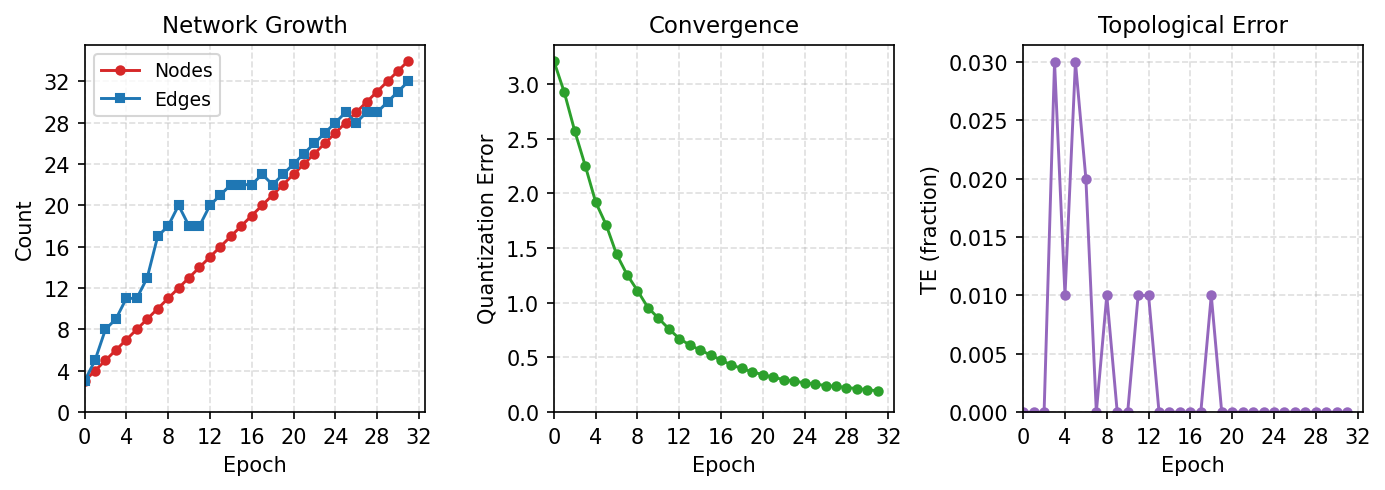
\includegraphics[width=0.92\linewidth]{two_moons_training.png}
\end{tikzfigure}
}

% ---------- Conclusion ----------
\block{Conclusion}{
\large
A \kw{fully integer, sub-10K-LUT FPGA GNG} engine. Edge-cell encoding
\hl{halves edge storage}; the fused pass merges decay, aging, and adaptation
into one sweep. Q8/Q16 fixed-point preserves low QE/TE with
\kw{deterministic latency} --- a hardware foundation for \kw{continual
self-organizing clustering at the edge}.
\vspace{2mm}\\
\small Supported by JST Moonshot R\&D, grant JPMJMS2034.\hfill
\textbf{Code:} github.com/ (fpga\_gng repo)
}

\end{columns}
\end{document}
